
%     %%%%%%%%%%%%%%%
%
%     P A C K A G E S
%
%     %%%%%%%%%%%%%%%

\documentclass[11pt, a4paper]{article}
\usepackage{fontspec}
\usepackage{caption}
\usepackage{mathtools}
\usepackage{gensymb}
\usepackage{float}
\usepackage{algorithmic}

% DOCUMENT LAYOUT
\usepackage{geometry}
\geometry{a4paper, textwidth=42em, textheight=70em, marginparsep=0.5em, marginparwidth=3.5em}
\setlength\parindent{0em}
\setlength\parskip{0.75em}
\captionsetup{width=0.8\textwidth}

% FONTS
\usepackage[usenames,dvipsnames]{xcolor}
\usepackage{xunicode}
\usepackage{xltxtra}
\defaultfontfeatures{Mapping=tex-text}
%\setromanfont [Ligatures={Common}, Numbers={OldStyle}, Variant=01]{Linux Libertine O}
%\setmonofont[Scale=0.8]{Monaco}
%%% modified by Karol Kozioł for ShareLaTeX use
\setmainfont[
  Ligatures={Common}, Numbers={OldStyle}, Variant=01,
  BoldFont=LinLibertine_RB.otf,
  ItalicFont=LinLibertine_RI.otf,
  BoldItalicFont=LinLibertine_RBI.otf
]{LinLibertine_R.otf}
\setmonofont[Scale=0.8]{DejaVuSansMono.ttf}

% HEADINGS
\usepackage{sectsty}
\usepackage[normalem]{ulem}
\sectionfont{\mdseries\upshape\Large}
\subsectionfont{\mdseries\scshape\normalsize}
\subsubsectionfont{\mdseries\upshape\normalsize}

\renewenvironment{abstract}{%
{\mdseries\scshape\Large\abstractname}
\vspace{1em}\\
}{\par\noindent}


%\usepackage[superscript]{cite}


% LISTINGS
\usepackage{listings}
\usepackage{color}
\usepackage{appendix}

\usepackage{color}
\definecolor{codered}{rgb}{0.61,0.21,0.18}
\definecolor{codegreen}{rgb}{0,0.6,0}
\definecolor{codegray}{rgb}{0.5,0.5,0.5}
\definecolor{codepurple}{rgb}{0.58,0,0.82}
\definecolor{backcolour}{rgb}{1.0,1.0,1.0}
\lstset{
  backgroundcolor=\color{backcolour},   
  commentstyle=\color{codegray},
  keywordstyle=\color{codered},
  numberstyle=\tiny\color{codegreen},
  stringstyle=\color{codepurple},
  basicstyle=\footnotesize\ttfamily,        % the size of the fonts that are used for the code
  breaklines=true,                          % sets automatic line breaking
  keepspaces=true,                          % keeps spaces in text, useful for keeping indentation of code
  showspaces=false,                         % show spaces everywhere adding particular underscores; it overrides 'showstringspaces'
  showstringspaces=false,                   % underline spaces within strings only
  showtabs=false,                           % show tabs within strings adding particular underscores
  stepnumber=2,                             % the step between two line-numbers. If it's 1, each line will be numbered
  tabsize=4, 	                            % sets default tabsize to 2 spaces
  title=\lstname                            % show the filename of files included with \lstinputlisting
}



%     %%%%%%%%%%%%%%%
%
%     D O C U M E N T
%
%     %%%%%%%%%%%%%%%


\begin{document}
\title{IAR Task 3 Final Report}
\author{Angus Pearson -- s1311631\\ Jevgenij Zubovskij -- s1346981}
\date{\today}
\maketitle

%       ^v^v^v^v^v^v^v^v^v^v^v^v^v^v^v^v^v^v^v^v^v^v^v^v^v^v^v^v^v^v^v^v^v^v^v^


\begin{abstract}
% the agency required by the task of exploring, discovering food and returning it to the robot's nest.
Given a \textit{Khepera II} robot with no prior knowledge of it's environment, we are able to 
simultaneously localise and map, under the assumption that the world is static.
This is built atop stochastic \textit{Adaptive Monte Carlo Localisation} \cite{principlesrobot} 
to correct compound localisation error, and a dyanmical \textit{Occupancy Grid} generation architecture, 
the combination of which constitute a SLAM system. The task requirement of food collection
behaviour is implemented using an \textit{A* search} planner.

Our existing Architecture from the previous IAR Assignments \cite{task1_report}\cite{task2_report} is further
extended, building upon the reactive behaviour, Redis datastore and ROS/Rviz real-time 
visualisation.

\end{abstract}


%       ^v^v^v^v^v^v^v^v^v^v^v^v^v^v^v^v^v^v^v^v^v^v^v^v^v^v^v^v^v^v^v^v^v^v^v^


\section{Dynamical Occupancy Grid}

We build up a map (occupancy grid) of the environment as the robot explores, where at time $0$, the map
is empty. In this implementation, the dimensions of the grid are effectively infinite, as there are
mechanisms allowing for automatic expansion in the even of the robot leaving the soft boundaries of
the grid. The grid is stored as a hashmap in Redis, not a 2D array, with missing keys being assumed 
unoccupied. This allows for rapid querying of arbitary cells' occupancy, and expanding the grid
is trivial given no keys need be updated.

However, a grid resize effectively invalidates any 2D cached array version of the map, all clients 
would be required to re-sync with Redis. To mitigate this, the grid's initial soft-dimensions
are large, as a cache reload is time-expensive.

The Occupancy grid is probabilistic, meaning each cell's occupancy is an integer in the range 
${[0..100]}$, with $0$ indicating certainly unoccupied, and $100$ indicating a certain occupation.

In our testing TODO

\subsection{Ray Tracing}

As the \textit{Khepera's} IR Range sensors give us the distance between the sensor and an object,
we can first transform this information from the robot's reference frame to the global (map)
reference frame, using a \textit{Transformation Matrix}:

\begin{equation}
  \begin{pmatrix}
    x_{map} \\
    y_{map}
  \end{pmatrix} = 
  \begin{pmatrix} 
    cos\Theta & sin\Theta \\
    -sin\Theta & cos\Theta
  \end{pmatrix}
  \cdot
  \begin{pmatrix}
    x_{robot} \\
    y_{robot}
  \end{pmatrix}
\end{equation}

Then using \textit{Bresenham's Line Algorithm} \cite{raytracealgo} we can raytrace between the
robot's position and the cell that we are seeing an object in; All the cells on this ray are 
updated -- If we've never seen before, they're marked as unoccupied, or if they are already 
marked in the map, the cell's value is updated to $0.9\times$ its value, given we now believe
it to be unoccupied. Backing off from a certain occpancy helps remove noise from the grid though
must be done conservatively to allow the localisation algorithm to make corrections.
An occupancy grid of the task environment evolved by this process is shown 
in Figure \ref{fig:occupancygrid}.

Grid population is done asynchronously from the main control loop, on an event-driven basis --
map updates are made as the control loop \textit{publishes} pose and sensory updtaes to Redis.

\begin{figure}[h]
  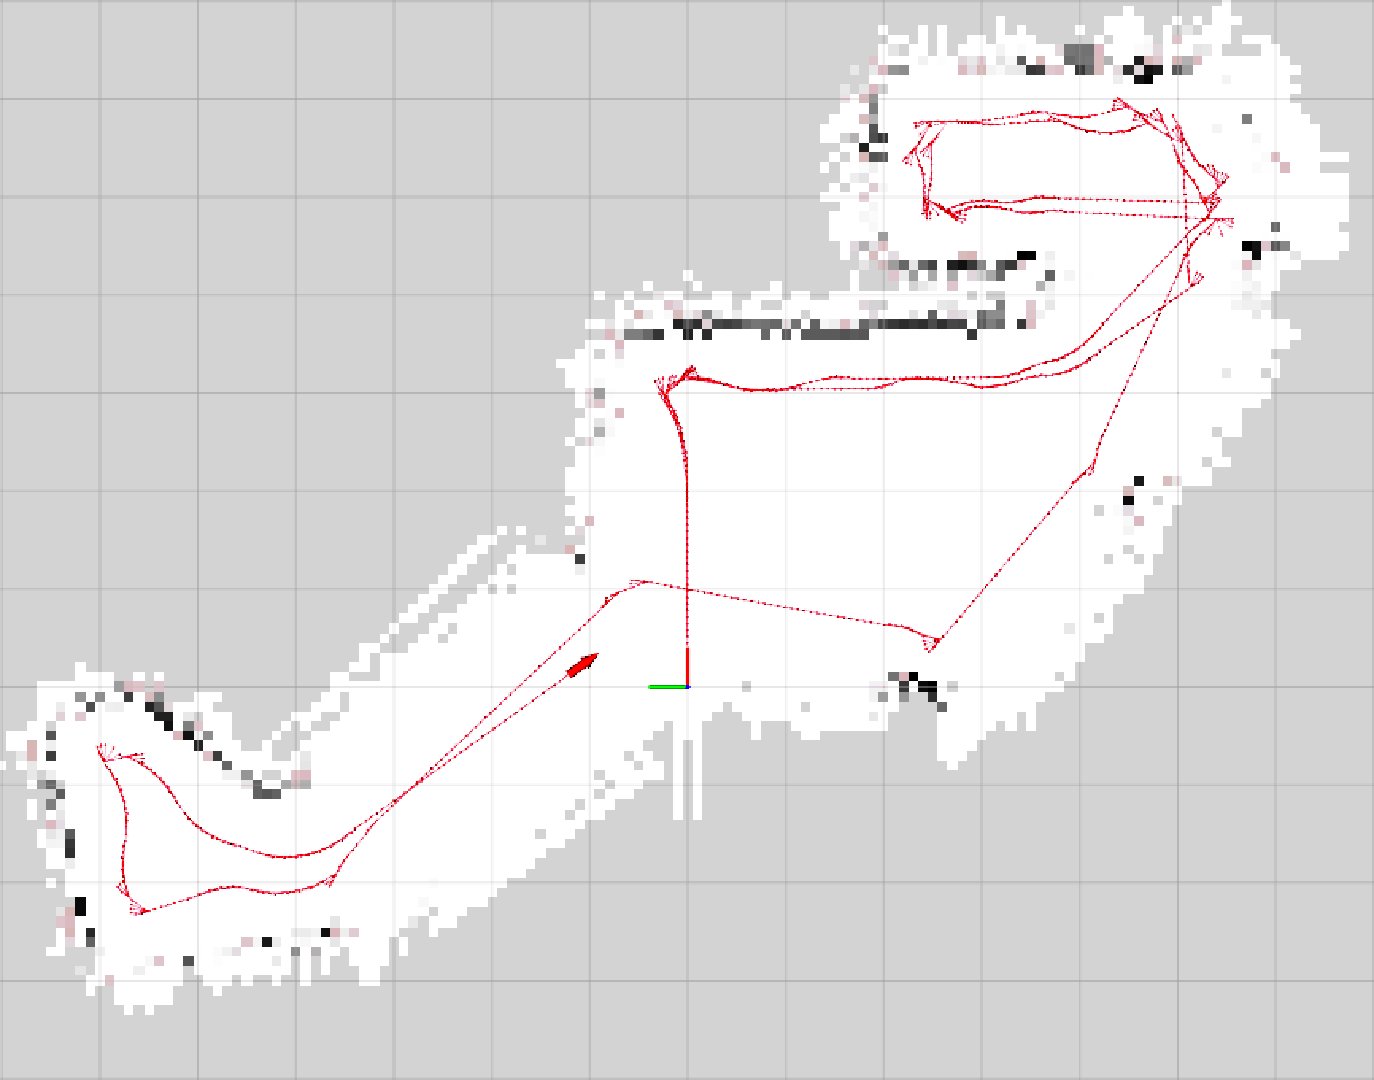
\includegraphics[width=\textwidth]{../assets/early-occupancy-grid-rviz.png}
  \caption{
    \label{fig:occupancygrid}
    Occupancy grid, with overlaid pose (large red arrow) and Odometry Trail (smaller magenta arrows).
    Black indicates occupancy, white free space. Grey regions are not present in the Occupancy Grid.
  }
\end{figure}



%       ^v^v^v^v^v^v^v^v^v^v^v^v^v^v^v^v^v^v^v^v^v^v^v^v^v^v^v^v^v^v^v^v^v^v^v^


\section{Adaptive Monte-Carlo Localisation}\label{sec:amcl}

\begin{figure}[h]
  \begin{center}
    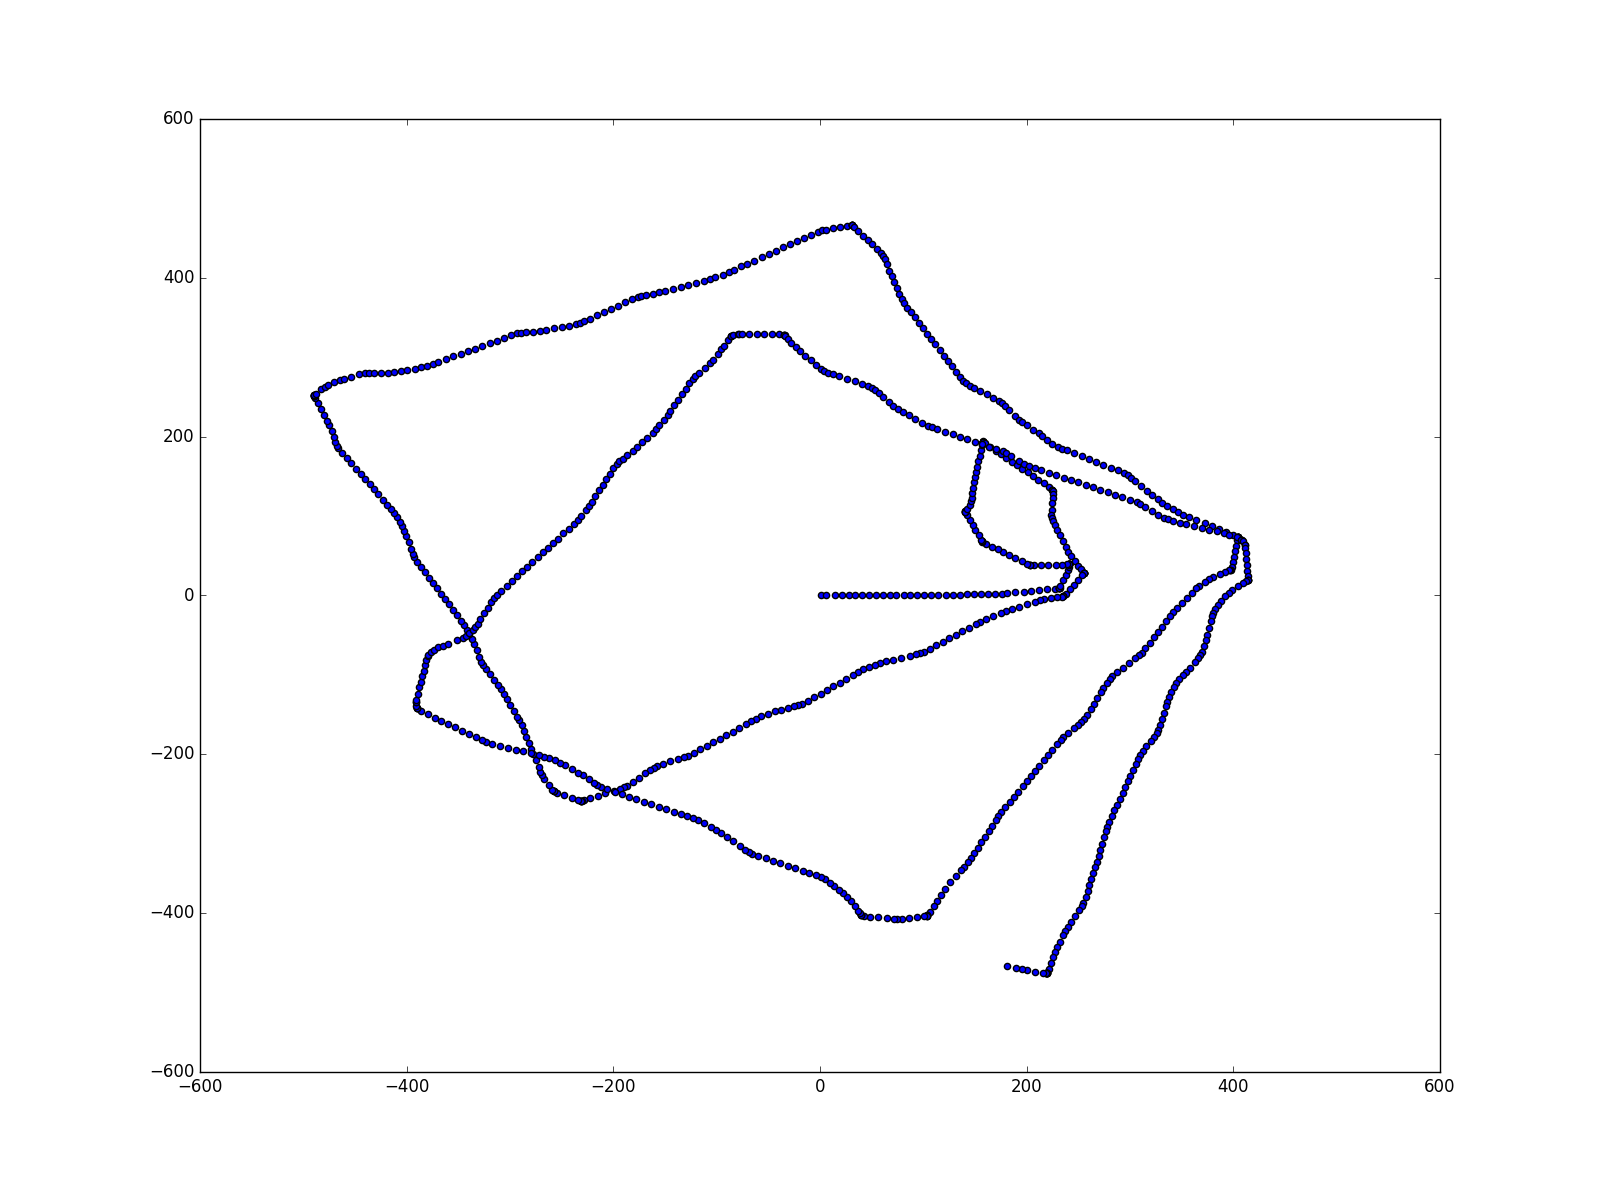
\includegraphics[width=0.7\textwidth]{../assets/plots/figure_1-3.png}
  \end{center}
  \caption{
    \label{fig:odometry_drift}
    Illustration of Odometry error. The robot was following the border of a simple square
    environment, but the trace of it's path shows a spiral instead. Axes are ${(x,y)}$
    coordinates in mm.
  }
\end{figure}

The existing system carried forward from \textit{Task 2} \cite{task2_report} maintained a pose estimate
that at each control loop epoch was updated by a discrete sensor model for the \textit{Khepera's} 
odometry. This model has no facility to model the compound error inherent to dead-reckoning with
odometry and as the robot continues to move in it's environment the belief about where the robot is quicky 
diverges from reality. As the task requires multiple excursions and returns to within 10cm of the nest,
this simple method alone is ineffective for localising the robot. This inherent drift is illustrated by
Figure \ref{fig:odometry_drift}.

The \textit{Adaptive Monte-Carlo Localisation} Algorithm as outlined in 
\textit{Probabilistic Robotics} \cite{probabilisticrobot} provides a stochastic method of correcting
for compound error and localising on an Occupancy Grid:

\textbf{\large Algorithm AMCL${(X_{t-1}, u_t, z_t)}$:}
\algsetup{indent=2em}
\begin{algorithmic}
  \STATE{$\bar{X_{t}}=X_{t}=\emptyset$}
  \FOR{$m=1$ \TO $M$}
  \STATE $x_{t}^{[m]}= \textrm{motion\_update}(u_{t},x_{(t-1)}^{[m]})$
  \STATE $w_{t}^{[m]}= \textrm{sensor\_update}(z_{t},x_{t}^{[m]})$
  \STATE $\bar{X_{t}}=\bar{X_{t}}+\langle x_{t}^{[m]},w_{t}^{[m]}\rangle $
  \ENDFOR
  \FOR{$m=1$ \TO $M$}
  \STATE $\textrm{draw } x_{t}^{[m]} \textrm{ from } \bar{X_{t}} \textrm{ with probability } \propto w_{t}^{[m]}$
  \STATE $X_{t}=X_{t}+x_{t}^{[m]}$
  \ENDFOR
  \RETURN $X_{t}$
\end{algorithmic}

Particles, which are Normally distributed samples of the Probability Density function of the robot's 
pose space, each representing a hypothesis about the robot's pose are drawn from the prior set 
of particles ${X_{t-1}}$ of size $M$ using the \textit{Weighted Reservoir 
Sampling Algorithm} \cite{reservoirsample}, the effect of which is that particles with greater 
weight ${w_t^{[m]}}$ (i.e. the more probable hypotheses) have a greater chance of persisting once 
or multiple times in the new set of particles ${X_t}$. Note that the number of particles remains 
the same at all times.

100 particles are used in this implementation; The compute time for the \textit{AMCL} grows quicky
as the number of particles increases. Further to this, while Redis affords flexibility, data persistence
and fanciness such as replaying a robot's trajectory, it presents a much larger overhead per lookup
or operation than a native datastructure. A naive \textit{sensor\_update} function will query
around 7500 occupancy grid cells in the vicinity of the robot: For each particle, each sensor is 
raytraced and then each grid cell on the rasterised ray is queried. Using a rather cool pre-fetching
and de-duplication algorithm in the sensor update (\texttt{mapping.py, Particles.update()}) the number
of unique queried cells is reduced to a nominal value of 54. These queries are serialised and
transacted as a batch job reducing network overhead.

These optimisations result in a 3.8 second to 0.08 second speedup (roughly $50\times$) compared to
the naive implementation, allowing the particle filter to run at every control loop cycle.

\begin{figure}[h]
  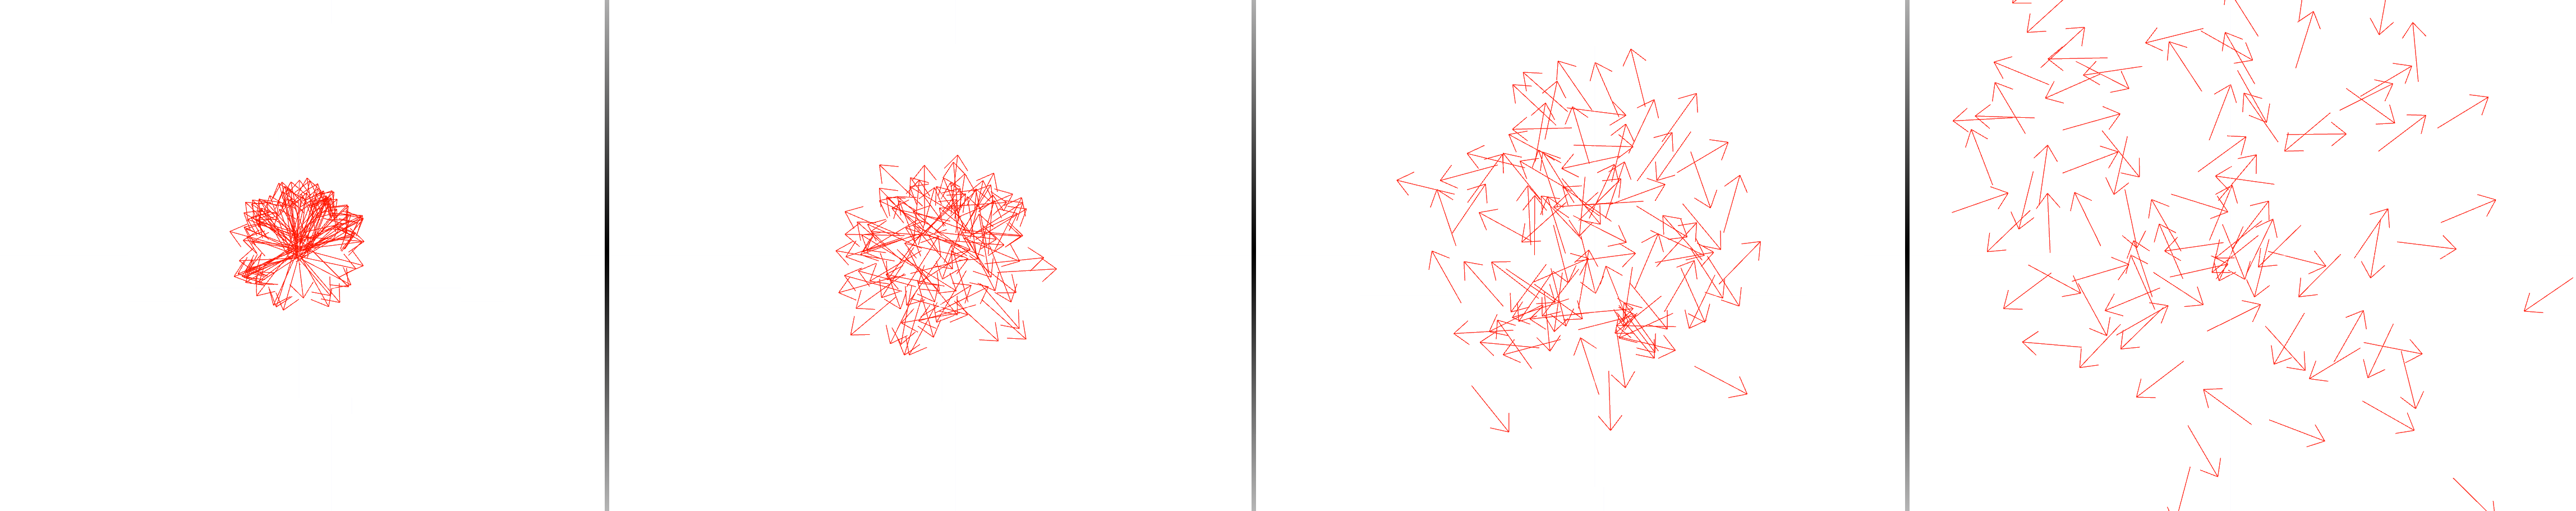
\includegraphics[width=\textwidth]{../assets/particle-disperse-random.png}
  \caption{
    \label{fig:particle-disperse}
    Dispertion of Particles by Monte Carlo method, from left to right with increasing time and 
    a particularly high gain (i.e. each epoch disperses the particles greatly, assuming very large error)
  }
\end{figure}

Figure \ref{fig:particle-disperse} illustrates how particles progressively diverge from the initial 
hypothesis, ${X_0}$. In our case, dynamical mapping affords a completely certain initial hypothesis
given the co-ordinate system is relative to said starting position; This prevents the need to
evenly distribute the particles over the environment at startup, so confidence in early localisations
is high with no multimodal properties.

\subsection{Limitations}

The environment for the task has many open areas, where the nearest objects are further away
than the robot can see. As the robot crosses one of these areas, the localisation error (the 
weighted varience of the particles) increases. If a new obstacle is encountered, by nature of the 
Occupancy Grid population rules the error at that time in the localisation will be directly transferred 
into the map as a misplaced set of occupied cells. Later relocalisations will take on part of this error.

Mitigations to this include constraining the robot to maneuvering `in view' of an obstacle at all times;
the bug behaviours from earlier tasks provide this to an extent but can't protect against error
when in free space.


%       ^v^v^v^v^v^v^v^v^v^v^v^v^v^v^v^v^v^v^v^v^v^v^v^v^v^v^v^v^v^v^v^v^v^v^v^

\newpage
\section{Planning}

With SLAM we can assume that our localisation is accurate and proceed to the primary goal -- gathering 
the maximum amount of food per unit time. For that we need to be able to plan out actions, which involves 
calculating routes to navigate the world and sequincing them accordingly.

\subsection{Path Planning Space}
\label{Path_Planning_Space}

\textit{(Path) Planning Space} is a term used  in this report to denote the representation of the 
physical world as the planner sees it, in this case $(x, y, \Theta)$. The existing use of this
pose representation from Task 1 \& 2 informs the choice of \textit{Path Planning Algorithm 
(\S\ref{Path_Planning_Algorithm})}. 

\subsubsection{Method Chosen}

The main methods of for planning over this representation are: \cite{path_space}

\begin{itemize}
	\item \textit{Occupancy Grid}
	\item \textit{Graph (Topological Map)}
\end{itemize}


The difference between these two from the perspective of planning is the efficiency of algorithm working 
on the data and the pre-processing as it goes into the algorithm. Because out Occupancy Grid is stored 
on a \textit{Redis Server} and it has very fine resolution (aka granularity), the number of grid 
squares (referred to as \textit{Grid Cells}) is immense. To obtain a graph representation of the
planning space at each epoch for the map at the resolution of the grid as implemented is
intractable from a compute time perspective.

Therefore planning over the Occupancy Grid is selected in preference to an abstracted representation
such as a topological map.

\subsubsection{Alterations}

The granularity of the \textit{Planning Grid (Planning Space)} did not necessarily have to match that 
of the occupancy grid on Redis for the following reasons:

\begin{itemize}

	\item Robot Dimensions     - the robot's dimensions are larger than the mapping (server-side) 
granularity
	\item Odometry Distortion  - extremely finely planned path on an occupancy grid introduces many 
turns, increasing odometry drift rate considerably \cite{task2_report}
	\item Runtime Optimization - a coarser grid reduces the depth of a given plan over the same route,
whilst sacrificing physical parity of said plan

\end{itemize}

The planning granularity is configurable though by default takes the same resolution as the Occupancy Grid.

Moreover, the \textit{(Grid) Cells} store their actual $(x ,y)$ coordinates as well as occupancy - whether 
they are free space or not. Grid cells are stored in a two dimensional array which is indexed into using 
actual $(x ,y)$ coordinates. Furthermore, said array is also dynamycally expandable in both dimensions so
as to accomodate any number of cells (limited only by memory capacity) in order to not miss a valid 
optimal path due to any array bounds which also makes this solution more extensible and easily modifiable.

A local cache of the Occupancy Grid to make planning more performant. As already noted calling out to 
the Redis server at a high rate incurrs a large overhead - a cached version can be used to plan
without convern for access frequency.


%       ^v^v^v^v^v^v^v^v^v^v^v^v^v^v^v^v^v^v^v^v^v^v^v^v^v^v^v^v^v^v^v^v^v^v^v^


\subsection{Path Planning Algorithm}
\label{Path_Planning_Algorithm}

This method should allow the robot to navigate the mapped space between any two unoccupied \textit{Cells} \textit{\S\ref{Code}} of the planning space.

\subsubsection{Research}

Firstly, there are many options for the \textit{Path Planning Algorithm} that search for a path between a goal and a destination location:

\begin{itemize}

	\item \textit{Floyd-Warshall Algorithm} \cite{path_warshall} - a many-to-many algorithm for planning routes
	\item \textit{Djikstra Graph Search Algorithm} \cite{path_djikstra} - a one-to-many algorithm
	\item \textit{A* Search Algorithm} \cite{path_astar}	- a one-to-one algorithm

\end{itemize}

These are some of the most common and robust algorihtms used in path planning. However, even based on 
the information above it can be concluded that Floyd-Warshall algorithm is not what we were looking 
because we have a single starting point - the position of the robot. Moreover, empirical data 
\cite{path_efficiency} shows that the best-first search algorithm is considerably faster than 
the Djikstra algorithm and in fact is in general considered one of the fastest planning algorithms -- 
it's variations as well as it's purest form are used industry-wide in robotics. 
More reasons for choosing A* are outlined in \textit{\S\ref{Path_Planning_Algorihtm_Alterations}}

\subsubsection{Method Chosen} 

A* was chosen for path calculation to the target grid cell. The pseudocode explaining its basic operation is as follows:

\begin{figure}[H]
	  \centering 
	  \lstinputlisting[language=python]{../../astar_pseudo.py}\caption{The A* algorithm pseudocode\cite{path_astar_pseudocode} adapted to use the \textit{Planning Space} chosen - an occupancy grid }
\end{figure} 


\begin{figure}[H]
 	  \centering
          \lstinputlisting[language=python]{../../astar_path_reconstruction.py}\caption{The A* algorithm path reconstruction pseudocode\cite{path_astar_grid_no_grid} adapted to use the \textit{Planning Space} chosen - an occupancy grid }
\end{figure} 



\subsubsection{Alterations}
\label{Path_Planning_Algorihtm_Alterations}

The chosen \textit{Path Planning Algorihtm - A*} (\S\ref{Path_Planning_Algorithm}) uses the movement 
and \textit{Heuristic Cost} to estimate the total cost of  including cell into the claculated path. 
As we know the pose of each grid cell, \textit{Euclidian Distances} were chosen to be a 
measure of transition cost between cells making it the cost function betwen any two cells $A$ and $B$. 
The \textit{Heuristic Function (Cost)} is $10$ times the Euclidian distance from currently considered 
cell to the goal. The reason for such a high number is that we wish to see the algorithm converge as 
fast as possible while finding an adequately short path to the desired destination which also reduces 
the amount of Redis Server requests for unknown occupancies. As a side note, the movement cost is 
simply the sum euclidian distances between nodes along the (considered) path involving said cell.

Secondly, the A* pseudocode had to be adapted to work on a grid instead of a graph which was solved 
by a simple function obtaining its neighbours by using the considered cell's pose to get its adjacent 
ones from the \textit{\S\ref{Path_Planning_Space} Occupancy Grid}.

Most iterations of the A* algorithm rely on either graphs \cite{path_astar_grid_no_grid}  or 
only movements up, down, left or right \cite{path_astar_grid_no_diagonals}. However, it seemed like a 
wasted opportunity to not allow the robot to move diagonally. Such cells are referred to as  
\textit{Diagonal Cells} - cells diagonal to the currently considered cell - whose adjacent cells 
we wish to consider for furhter pathing. The scenario where the diagonal cell is blocked by two of 
its neighbours must be accounted for. In this case the diagonal cell can no longer participate in 
path calculation as shown in the Figure \ref{fig:diagonalcell}


\begin{figure}[H]
	  \centering
	  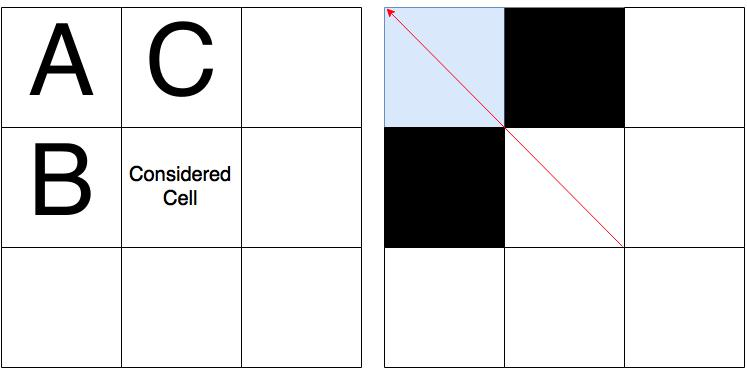
\includegraphics[width=30em]{../assets/fig_astar_diagonal.jpg}
          \caption{
            \label{fig:diagonalcell}
            The \textbf{left} figure shows the $central$ cell (square) is the so called \textit{Considered Cell} whose neighbours we are trying to obtain to plan a path. The \textbf{left} figure shows that we cannot consider the \textit{Diagonal Cell} $A$ as a valid neighbour because it is blocked by $B$ and $C$ making the movement along the red arrow as seen in the \textbf{right} figure impossible}
\end{figure} 






%       ^v^v^v^v^v^v^v^v^v^v^v^v^v^v^v^v^v^v^v^v^v^v^v^v^v^v^v^v^v^v^v^v^v^v^v^



\subsection{The Planner}

This section is concerned with the intergation of the algorithm and data structures described above 
into the main control loop and its interaction with previosuly established subsystems 
\cite{task2_report}. The algorithm determining the next action or travel destination and sequencing 
the execution of said action is called the \textit{Planner} and is, therefore, responsible for 
maximizing the food collection rate by sequencing events governing said rate.

\subsubsection{Method Chosen}
\label{Planner_Principle}

Now that we are able to localize ourselves, know the map and can calculate paths on the planning 
grid, we can set priorites for action to maximize food gathering. Firstly, it is important to 
note that each \textit{Food Source} has only one unit of \textit{Food}. 
Upon return to the \textit{Nest} and dropping off currently collected food the planner resets the 
food sources which now have food units again, starting a new \textit{Food Collection 
Round (a.k.a. Round)}. Action priorites were set as follows:

\begin{enumerate}
	\item \textit{Find} the first food source to begin periodic behavior in the following points
	\item \textit{Explore} once per Food Collection Round
	\item \textit{Collect} closest uncollected known / recorded food source
	\item \textit{Return} to the nest and drop off collected food
\end{enumerate}

We aim to find some food source early to be able start collecting food as soon as possible. 
Once this is done, exploration for new food sources becomes less of a priority and is only invoked 
once per round as we do not wish to waste too much time on exploration when we already have
a known location to collect from. Next on the list of priorities is collecting all the food before 
returning to the nest to drop it off.

\begin{figure}[H]
	  \centering
	  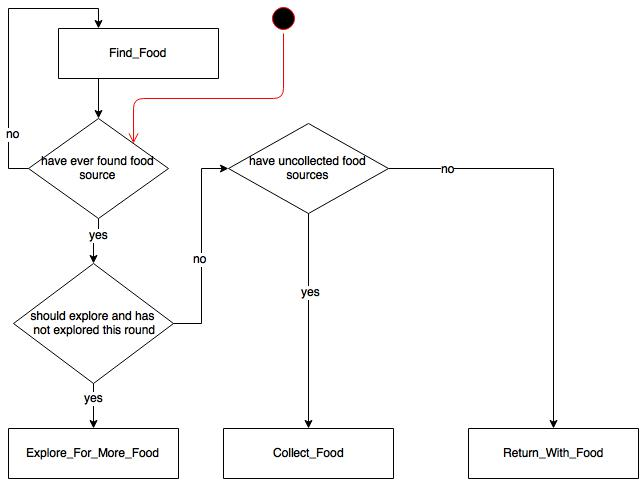
\includegraphics[width=0.9\textwidth]{../assets/fig_planner.jpg}
          \caption{The planning algorithm - the \textit{Planner} in control-flow form, this decision making tree is implored on every iteration of the control loop and determines the action the system is to follow.}
\end{figure} 

The robot aims to collect the closest food first (based on Euclidian distances). The movement 
between cells is moevement along the vector between their recorded coordinates by adjusting the 
angle along the \textit{Vector of Approach}, same as \textit{Return Algorithm}\cite{task2_report}. 
Moreover, sometimes unxecpected events can happen that coud lead the robot away from said approach 
vector. Hence, the next destination is decided (as per above priority list) when the following 
events happen:

\begin{itemize}

	\item Food collected from a Food Source
	\item Food dropped off at nest - round finished
	\item Path lost - went a distance over the threshold away from the path

\end{itemize}

\subsubsection{Alterations}
\label{Planner_Algorithm_Alterations}

After reviewing initial \textit{\S\ref{Experimental_Results} Experimental Results} it was decided 
that due to the grid granularity being set (by default) in the same order of magnitude as robot 
dimensions, it is reasonable to assume that no two food sources can exist in the same grid cell 
as the cell sizes are assumed to be set by the user / programmer to a granularity not exceeding 
robot dimensions. Lastly, because the algorithm needs to find new food sources, the boredom 
mechanism \cite{task1_report} was reinstated into the control loop and is the exploration 
mechanism and is utilized during the \textit{Find} stages of the algorithm.


%       ^v^v^v^v^v^v^v^v^v^v^v^v^v^v^v^v^v^v^v^v^v^v^v^v^v^v^v^v^v^v^v^v^v^v^v^


\subsection{User Input and Alterations}
\label{Planner_User_Input}

The user input of \textit{Space} being pressed is used to indicate the presence of a new food 
source being found. 

\subsection{Subsystem Interaction}

Lastly, the integration of the algorithm into the main system is seamless and practically mimics 
the integration of the \textit{Return Algorithm} \cite{task2_report} a.k.a. the \textit{Bug 2.4.1.1.2}. 
The difference is now we know where there are walls or free space. Hence, the robot can fully 
devolve control to the planner, unless we are exploring using "boredom" \cite{task2_report} or 
are being "unstuck" \cite{task2_report} without fear of the robot crashing into the wall. 

This amounts to SLAM and A* are the main control authority in the system, unless we need 
to avoid collision. A further note is that the above distinction is not as clear in the 
\textit{\S\ref{Code} Code} because of the location of methods, however, the end result 
(and aim) is as descibed above.


%       ^v^v^v^v^v^v^v^v^v^v^v^v^v^v^v^v^v^v^v^v^v^v^v^v^v^v^v^v^v^v^v^v^v^v^v^


\section{Experimental Results}
\label{Experimental_Results}






TODO make sure angus has a pic of waht an occupancy grid is
TODO comment somehow on the ganularity effect on performance (and do tests)
TODO make sure occupancy grid is already described in a previous section
TODO reference pictures
TODO set granularity to robot dimension
TODO insert stuff from google drive
TODO: Empirical results


TODO Rule the world



%       ^v^v^v^v^v^v^v^v^v^v^v^v^v^v^v^v^v^v^v^v^v^v^v^v^v^v^v^v^v^v^v^v^v^v^v^


\begin{thebibliography}{}

\bibitem{task1_report} 
\par{IAR 2016 Task1 Report}
\\
\textit{Angus Pearson, Jevgenij Zubovskij}

\bibitem{task2_report} 
\par{IAR 2016 Task2 Report}
\\
\textit{Angus Pearson, Jevgenij Zubovskij}


\bibitem{principlesrobot} % The bug one
\par{Principles of Robot Motion: Theory, Algorithms, and Implementation \S2.1 `Bug Algorithms'}
\\
\textit{Howie Choset}


\bibitem{probabilisticrobot} % The AMCL one
\par{Probabilistic Robotics (Intelligent Robotics and Autonomous Agents), MIT Press, 2005}
\\
\textit{Thrun, Sebastian and Burgard, Wolfram and Fox, Dieter}


\bibitem{reservoirsample}
\par{Reservoir Sampling, Dictionary of Algorithms and Data Structures}
\\
\textit{Black, Paul E. (26 January 2015)}


\bibitem{raytracealgo}
\par{A Linear Algorithm for Incremental Digital Display of Circular Arcs}
\\
\textit{Commun. ACM, J Bresenham, Feb. 1977}

\bibitem{path_space}
\par{Map Representation Comparison and Planning (online article)}
\\
\textit{http://correll.cs.colorado.edu/?p=965}



\bibitem{path_warshall} 
\par{Theory of Algorithms (lecture)}
\\
\textit{http://cs.winona.edu/lin/cs440/ch08-2.pdf}

\bibitem{path_djikstra} 
\par{Greedy Algorithms (online article)}
\\
\textit{http://www.geeksforgeeks.org/greedy-algorithms-set-6-dijkstras-shortest-path-algorithm/}

\bibitem{path_astar}
\par{A* Comparison (online article)}
\\
\textit{http://theory.stanford.edu/~amitp/GameProgramming/AStarComparison.html}

\bibitem{path_efficiency} 
\par{Comparative Study of Path Planning Algorithms}
\\
\textit{http://research.ijcaonline.org/volume39/number5/pxc3877058.pdf}

\bibitem{path_astar_pseudocode} 
\par{A* Search Algorithm (online article)}
\\
\textit{http://web.mit.edu/eranki/www/tutorials/search/}



\bibitem{path_astar_grid_no_diagonals} 
\par{Introduction to A* (online article)}
\\
\textit{http://theory.stanford.edu/~amitp/GameProgramming/AStarComparison.html}



\bibitem{path_astar_grid_no_grid} 
\par{A* Search Alogorith (online article)}
\\
\textit{https://en.wikipedia.org/wiki/A*\_search\_algorithm}




\end{thebibliography}

\newpage
\section*{Appendix}
\subsection{Code Listings}
\label{Code}
\lstinputlisting[language=python]{../../main.py}
\lstinputlisting[language=python]{../../data.py}
\lstinputlisting[language=python]{../../comms.py}
\lstinputlisting[language=python]{../../mapping.py}
\lstinputlisting[language=python]{../../state.py}
\lstinputlisting[language=python]{../../utils.py}
\lstinputlisting[language=python]{../../pathing_state.py}
\lstinputlisting[language=python]{../../pathing_algorithm.py}
\lstinputlisting[language=python]{../../astar.py}
\lstinputlisting[language=python]{../../navigation_state.py}
\lstinputlisting[language=python]{../../navigation_algorithm.py}
\lstinputlisting[language=python]{../../odometry_algorithm.py}
\lstinputlisting[language=python]{../../odometry_state.py}
\lstinputlisting[language=python]{../../constants.py}
\lstinputlisting{../../requirements.txt}
\lstinputlisting{../../redis-min.conf}



\end{document}
